\chapter{The response to selection}
Evolution by natural selection requires:
\begin{enumerate}
\item Variation in a phenotype
\item That survival is non-random with respect to this phenotypic
variation.
\item That this variation is heritable.
\end{enumerate}
Points 1 and 2 encapsulate our idea of Natural Selection, but evolution by natural
selection will only occur if the 3rd condition is met. It is the
heritable nature of variation that couples change within a generation
due to natural selection, to change across generations (evolutionary
change). \\

Lets start by thinking about the change within a generation due
to directional selection, where selection acts to change the mean
phenotype within a generation. For example, a decrease in mean height within a
generation, due to taller organisms having a lower chance of surviving
to reproduction than shorter organisms. Specifically, we'll denote our mean phenotype at
reproduction by $\mu_S$, i.e. after selection has acted, and our mean
phenotype before selection acts by $\mu_{BS}$. This second quantity may be hard to
measure, as obviously selection acts throughout the life-cycle, so it
might be easier to think of this as the mean phenotype if selection
hadn't acted. So the mean phenotype changes within a generation is $\mu_{S} - \mu_{BS}= S$.  \\

\begin{marginfigure}
\begin{center}
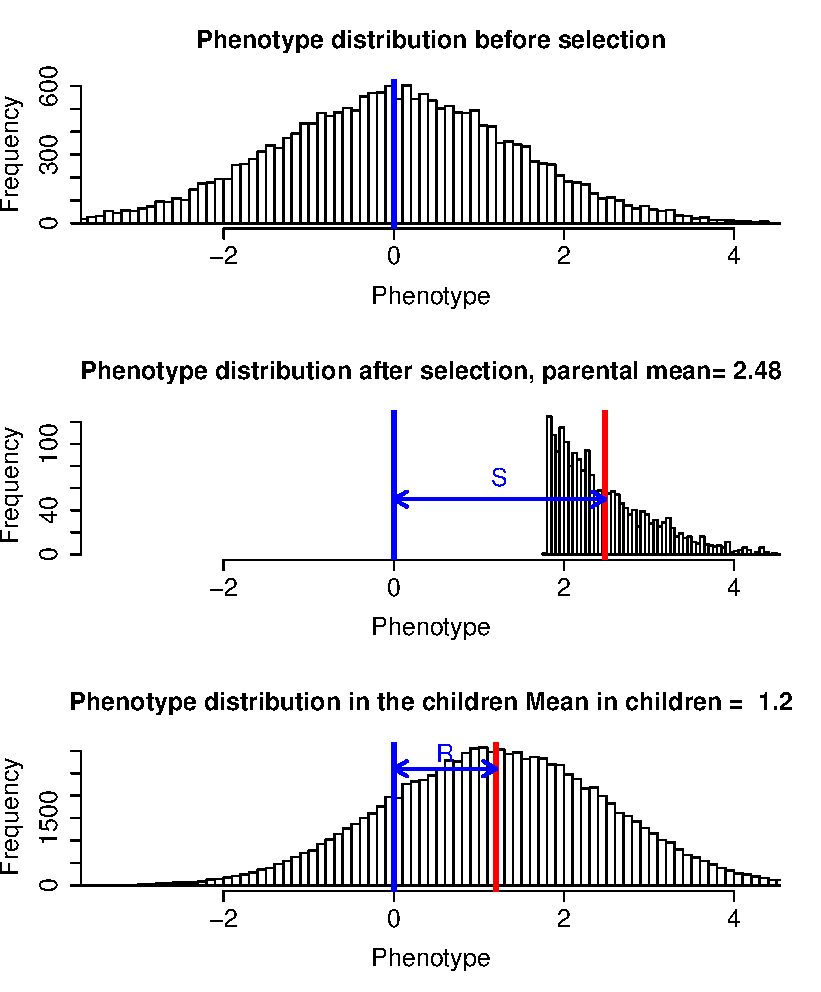
\includegraphics[width=\textwidth]{figures/Response_to_sel/QT3.pdf}
\end{center}
\caption{{\bf Top.} Distribution of phenotype in parental population
  prior to selection, $V_A=V_E=1$. {\bf Middle.} Only individuals in the top $10\%$
  of the phenotypic distribution are selected to reproduce, the shift
  in the phenotypic mean is $S$. {\bf Bottom.}  Phenotypical distribution of
  children of the selected parents, the shift in the mean phenotype is
$R. $}
\end{marginfigure}

We are interested in predicting the distribution of phenotypes in next
generation, in particular we are interested in the mean phenotype in
the next generation to understand how directional selection has
contributed to evolutionary change. We'll denote the mean phenotype in
offspring, i.e. the mean phenotype in the next generation before selection acts,
as $\mu_{NG}$. The change across generations we'll call the response
to selection $R$ and put this equal to $\mu_{NG}- \mu_{BS}$. \\


The mean phenotype in the next generation is
\begin{equation}
\mu_{NG} = \E \left( \E(X_{kid} | X_{mum},X_{dad}) \right)
\end{equation}
where the outer expectation is over the randomly mating of individuals
who survive to reproduce. We can use eqn. \ref{predict_kid} to obtain
an expression for this
\begin{equation}
\mu_{NG} = \mu_{BS} +
\beta_{mid,kid} ( \E(X_{mid}) - \mu_{BS})
\end{equation}

\begin{marginfigure}
\begin{center}
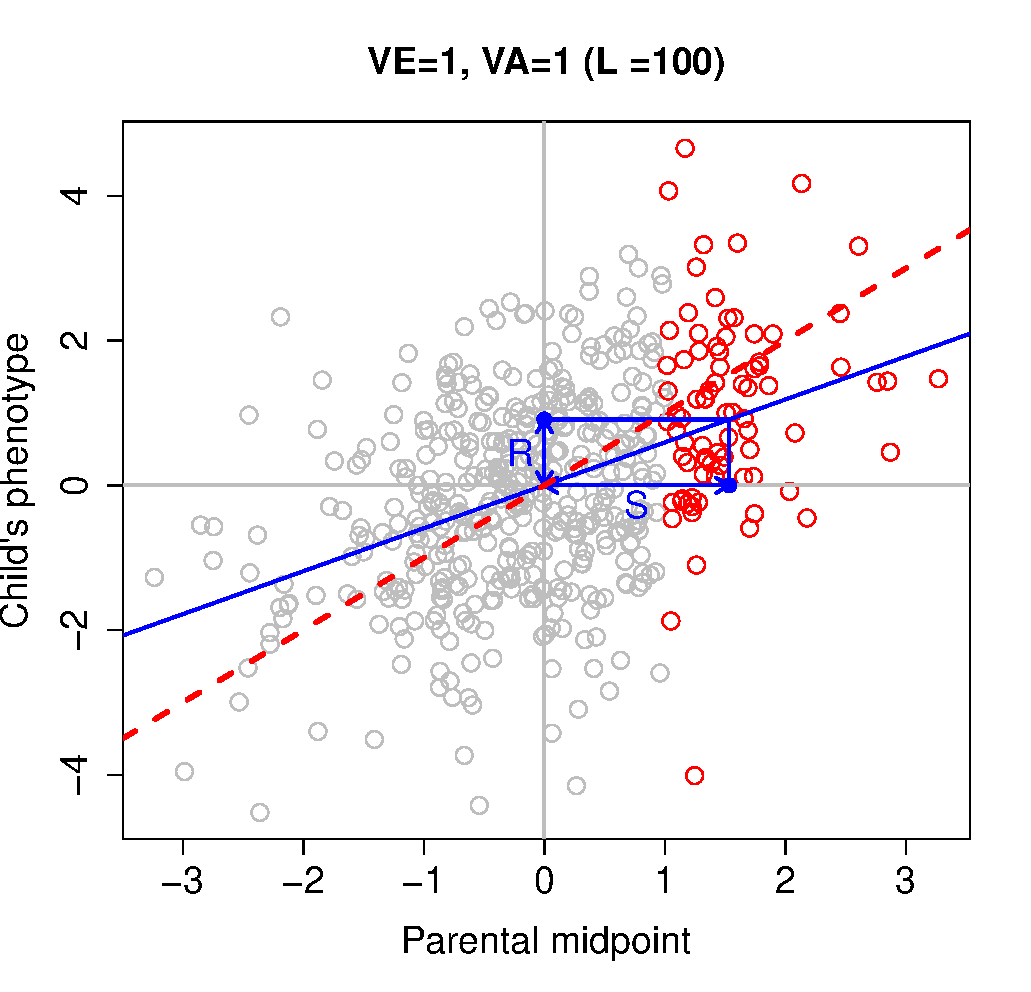
\includegraphics[width=\textwidth]{figures/Response_to_sel/Breeders_eqn.pdf}
\end{center}
\caption{A visual representation of the Breeder's equation. Regression of parental mid-point phenotype on child's
  phenotype ($V_A=V_E=1$). Under truncation selection only individuals
  (red) with phenotypes $>1$ are bred.}
\end{marginfigure}

so to obtain $\mu_{NG}$ we need to compute $\E(X_{mid})$ the expected
mid-point phenotype of pairs of individuals who survive to
reproduce. Well this is just the expected phenotype in the individuals
who survived to reproduce ($\mu_{S}$), so
\begin{equation}
\mu_{NG} = \mu_{BS} +
h^2 (\mu_S - \mu_{BS})
\end{equation}
So we can write our response to selection as
\begin{equation}
R = \mu_{NG} -\mu_{BS}  =
h^2 (\mu_S - \mu_{BS}) = h^2 S \label{breeders_eqn}
\end{equation}
So our response to selection is proportional to our selection
differential, and the constant of proportionality is the narrow sense
heritability. This equation is sometimes termed the Breeders
equation. It is a statement that the evolutionary change across
generations ($R$) is proportional to the change caused by directional selection
within a generation, and the strength of this relationship is
determined by the narrow sense heritability. \\

\graham{Lost the barncle question, put it back in.}


\marginnote{
\begin{question}
A population of red deer were trapped on Jersey (an island off of
England) during the last inter-glacial period. From the fossil record \cite{lister:89}
we can see that the population rapidly adapted to their new
conditions, within 6,000 years they evolved from an estimated mean weight of
the population of 200kg to an estimated mean weight of 36kg (a 6 fold
reduction)! You estimate that the generation time
of red deer is 5 years and, from a current day population, that the narrow sense heritability of the
phenotype is 0.5.\\
{\bf A)}	Estimate the mean change per generation in the mean body weight. \\

{\bf B)}	Estimate the change in mean body weight caused by
selection within a generation. State your assumptions.\\

{\bf C)}	Assuming we only have fossils from the founding population and the population after 6000 years, should we assume that the calculations accurately reflect what actually occurred within our population?
\end{question}
}

Using the fact that $h^2=V_A/V$ we can rewrite this in a different form as
\begin{equation}
R= V_A \frac{S}{V}
\end{equation}
i.e. our response to selection is the additive genetic variance of our
trait ($V_A$) multiplied by the change within a generation as a
fraction of the total phenotypic variance ($S/V$, sometimes called the
the selection gradient $\beta$).\\

\paragraph{The long-term response to selection}
If our selection pressure is sustained over many generations we can
use our breeders equation to predict the response. If we are willing
to assume that our heritability does not change and we maintain a constant selection
gradient, then after $n$ generations our phenotype mean will have
shifted 
\begin{equation}
n h^2 S
\end{equation}
i.e. our population will keep up a linear response to selection.


\paragraph{Alternative formulations of the Breeder's equation.}
A change in mean phenotype within a generation occurs because of the
differential fitness of our organisms. To think more carefully about this change within a
generation lets think about a simple fitness model where our phenotype affects the
viability of our organisms (i.e. the probability they survive to
reproduce). The probability that an individual has a phenotype $X$
before selection is $p(X)$, so that the mean phenotype before
selection is
\begin{equation}
\mu_{BS} = \E[X] =  \int_{-\infty}^{\infty} x p(x) dx
\end{equation}
The probability that an organism with a phenotype $X$ survives to
reproduce is $w(X)$, and we'll think about this as the fitness of
our organism. The probability distribution of phenotypes in those who
do survive to reproduce is
\begin{equation}
\P(X | \textrm{survive}) =  \frac{p(x) w(x)}{
\int_{-\infty}^{\infty} p(x) w(x) dx}.
\end{equation}
where the denominator is a normalization constant which ensures that
our phenotypic distribution integrates to one. The denominator also
has the interpretation of being the mean fitness of the population,
which we'll call $\wbar$, i.e.  
\begin{equation}
\wbar =  
\int_{-\infty}^{\infty} p(x) w(x) dx.
\end{equation}


Therefore, we can write the mean phenotype in those who survive to
reproduce as
\begin{equation}
\mu_S = \frac{1}{\wbar}\int_{-\infty}^{\infty} x p(x) w(x) dx
\end{equation}

If we mean center our population, i.e. set the phenotype before
selection to zero, then
\begin{equation}
S= \frac{1}{\wbar}\int_{-\infty}^{\infty} x p(x) w(x) dx
\end{equation}
if $\mu_S=0$.  Inspecting this more closely we can see that $S$ has
the form of a covariance between our phenotype $X$ and our fitness
$w(X)$ ($Cov(X,w(X))$). Thus our change in mean phenotype is directly a measure of the
covariance of our phenotype and our fitness. Rewriting our breeder's
equation using this observation we see
\begin{equation}
R = \frac{V_A}{V}  Cov(X,w(X))
\end{equation}
we see that the response to selection is due to the fact that our
fitness (viability) of our organisms/parents covaries with our phenotype, and
that our child's phenotype is correlated with the parent phenotype.

\subsection{The response of multiple traits to selection, the
  multivariate breeder's equation.}
We can generalize these results for multiple traits, to ask how selection on
multiple phenotypes plays out over short time intervals. We'll write
our change in the mean our multiple phenotypes within a generation as
the vector $\bf{S}$ and our response across multiple generations as
the vector $\bf{R}$. These two quantities are related by 
\begin{equation}
\bf{R} = \bf{G} \bf{V}^{-1} \bf{S} = \bf{G} \bf{\beta}
\end{equation}
 where $\bf{V}$ and $\bf{G}$ are our matrices of the
 variance-covariance of phenotypes and additive genetic values
 (eqn. \eqref{G_matrix} \eqref{P_matrix}) and
 $\bf{\beta}$ is a vector of selection gradients (i.e. the change
 within a generation as a fraction of the total phenotypic variance). \cite{lande:79}
To make this a bit more intuitive, consider two traits we are writing 
\begin{eqnarray}
R_1 & = V_{A,1} \beta_1 + V_{A,1,2} \beta_2 \nonumber \\
R_2 & = V_{A,2} \beta_2 + V_{A,1,2} \beta_1  \nonumber \\
\end{eqnarray}
where the $1$ and $2$ index our two different traits. This is a
statement that our response in any one phenotype is modified by
selection on other traits that covary with that trait.
This offers a good way to think about how genetic trade offs play out
over evolution over short time-scales.

\begin{marginfigure}[-40mm]
\begin{center}
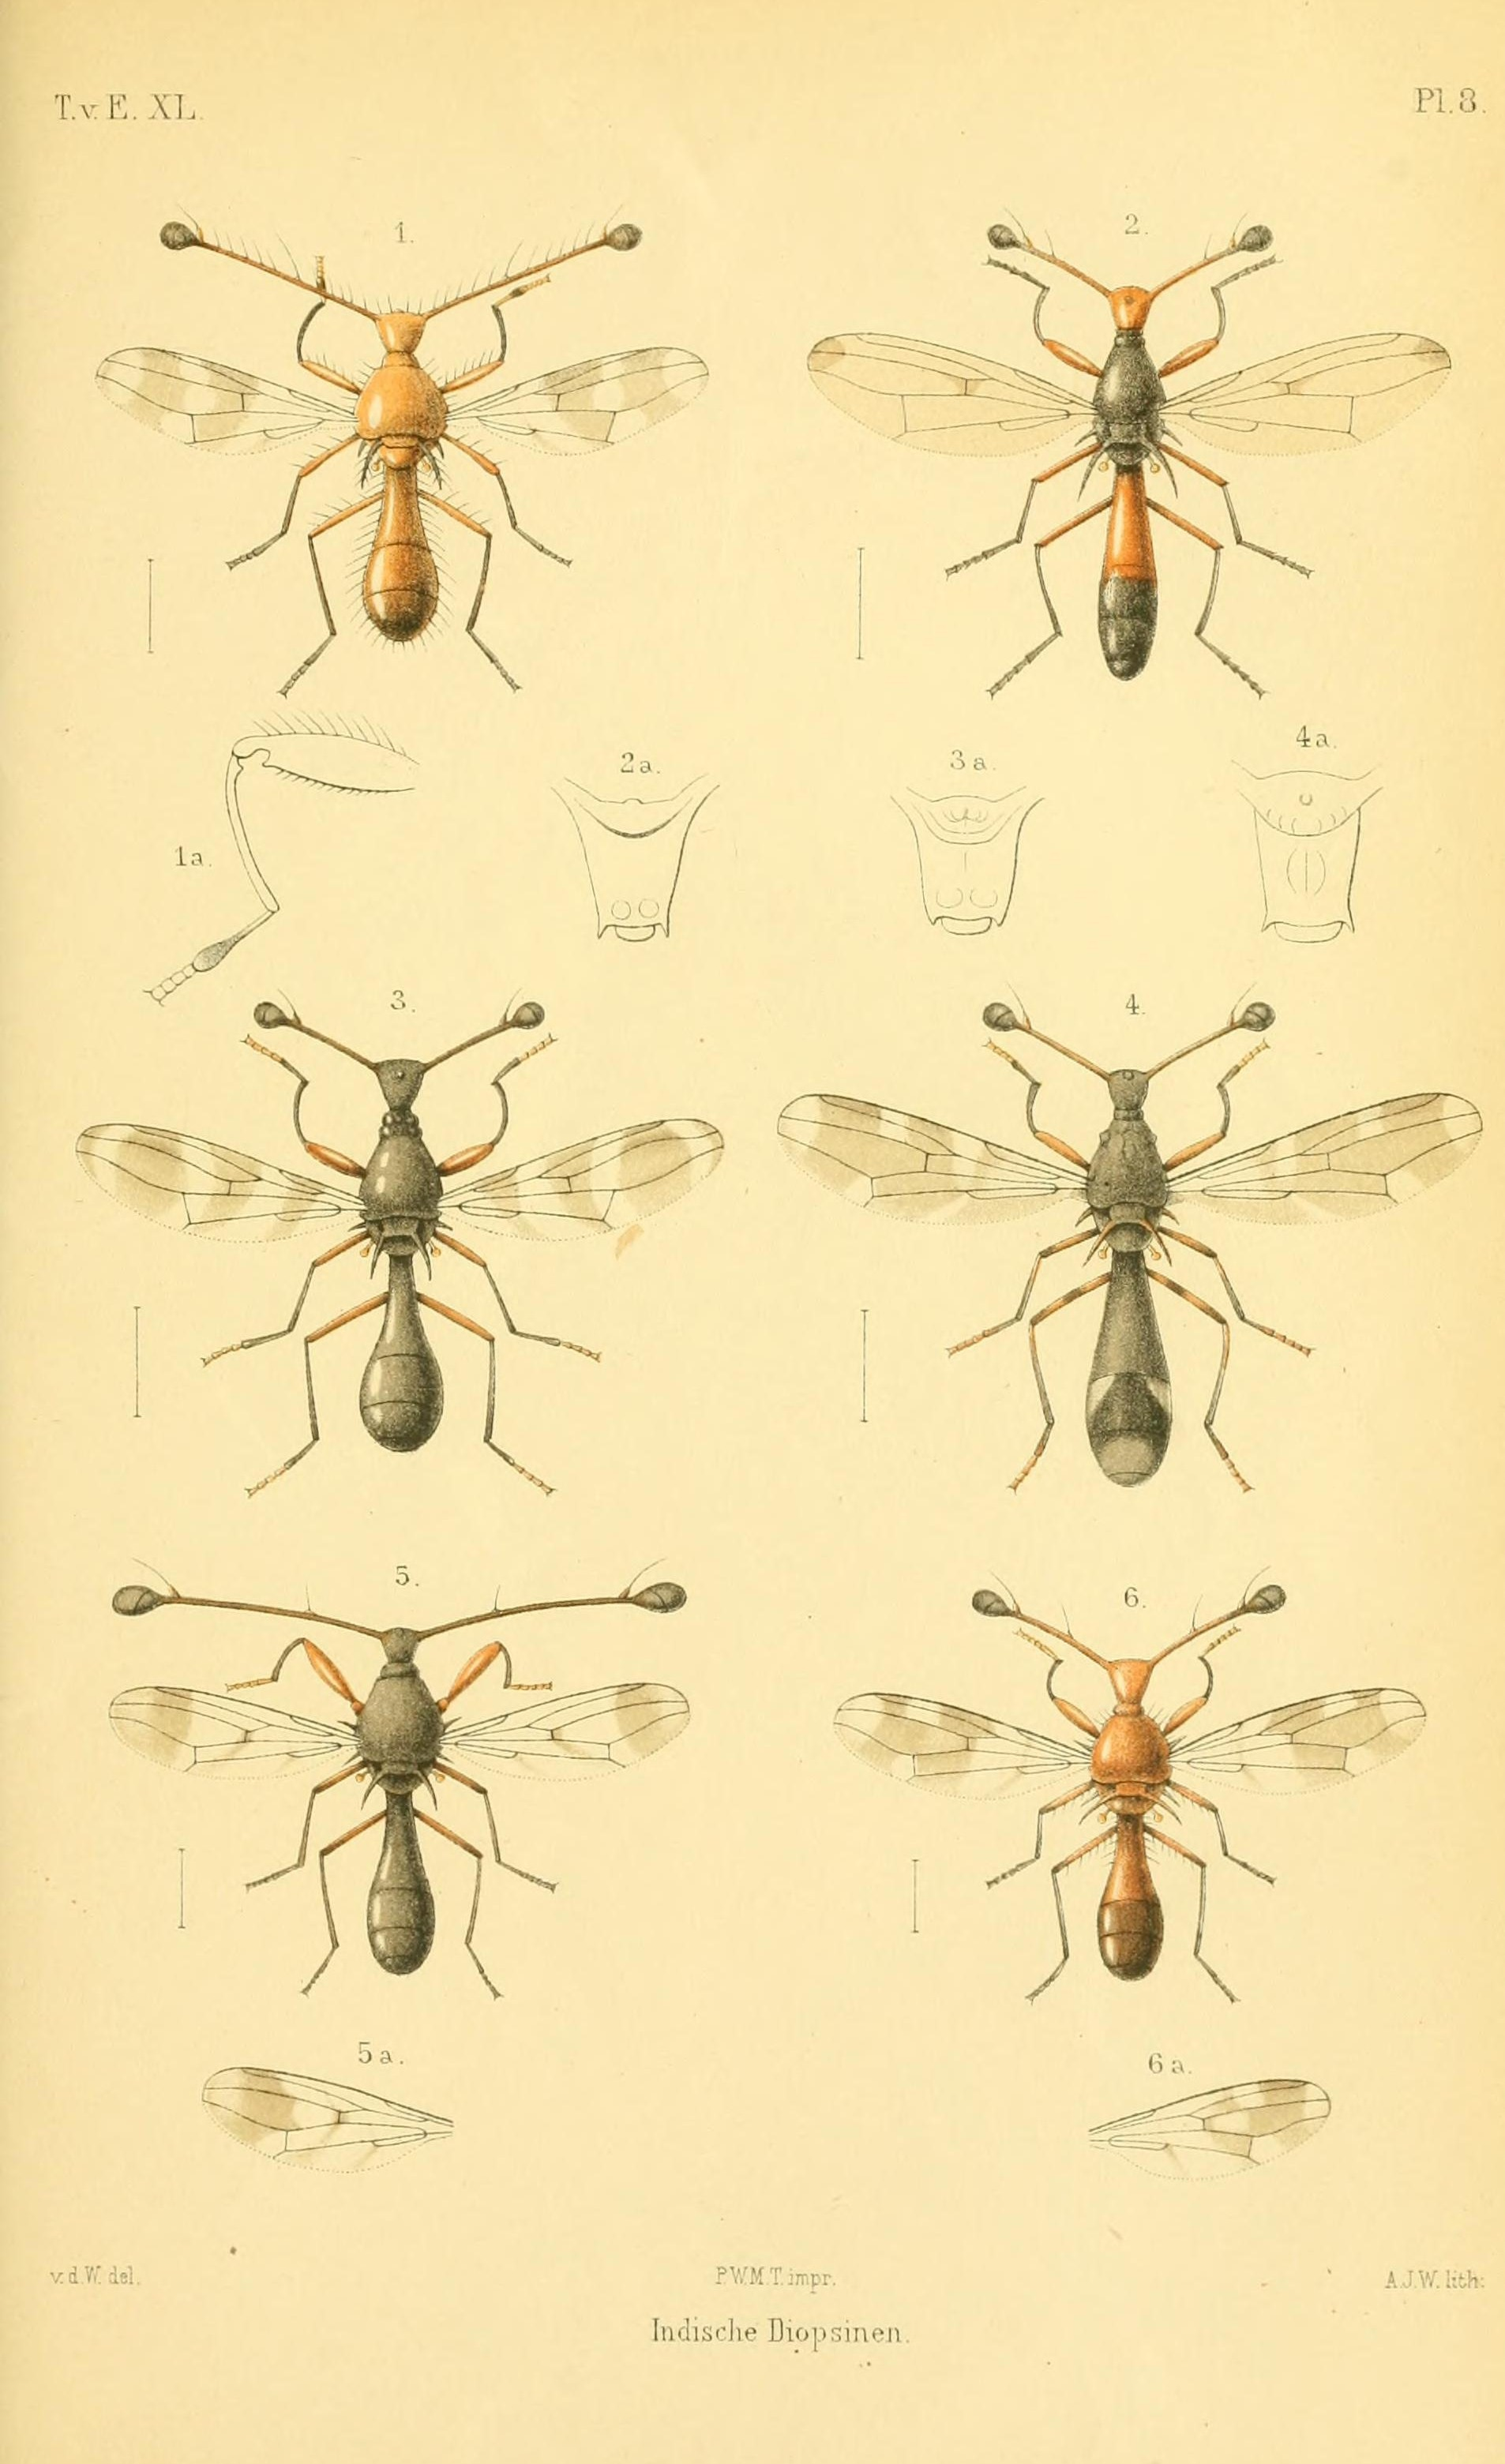
\includegraphics[width=0.9 \textwidth]{illustration_images/Quant_gen/Stalk_eyed_flies/WulpPlateVIIIjpg.jpg}
\end{center}
\caption{Stalk-eyed Flies ({\it Diopsidae}).  Diptera.
van der Wulp. 1898. BHL} \label{fig:Stalk_eyed_flies}  
\end{marginfigure}

As an example of correlated responses to selection consider the  \citeauthor{wilkinson:93} selection experiment on Stalk-eyed
 flies ({\it Cyrtodiopsis  dalmanni}). Stalk-eyed flies have evolved
 amazingly long eye-stalks. In the lab \citeauthor{wilkinson:93} established six populations of
 wild-caught flies and selected up and down on males eye-stalk to body
 size ratio for 10 generations (left plot in Figure
 \ref{fig:Stalk_eyed_response}). Despite the fact that he did not
 select on females, he saw a correlated response in the females from
 each of the lines (right plot), because the genetic correlation
 between male and female body proportions. 

\begin{figure}
\begin{center}
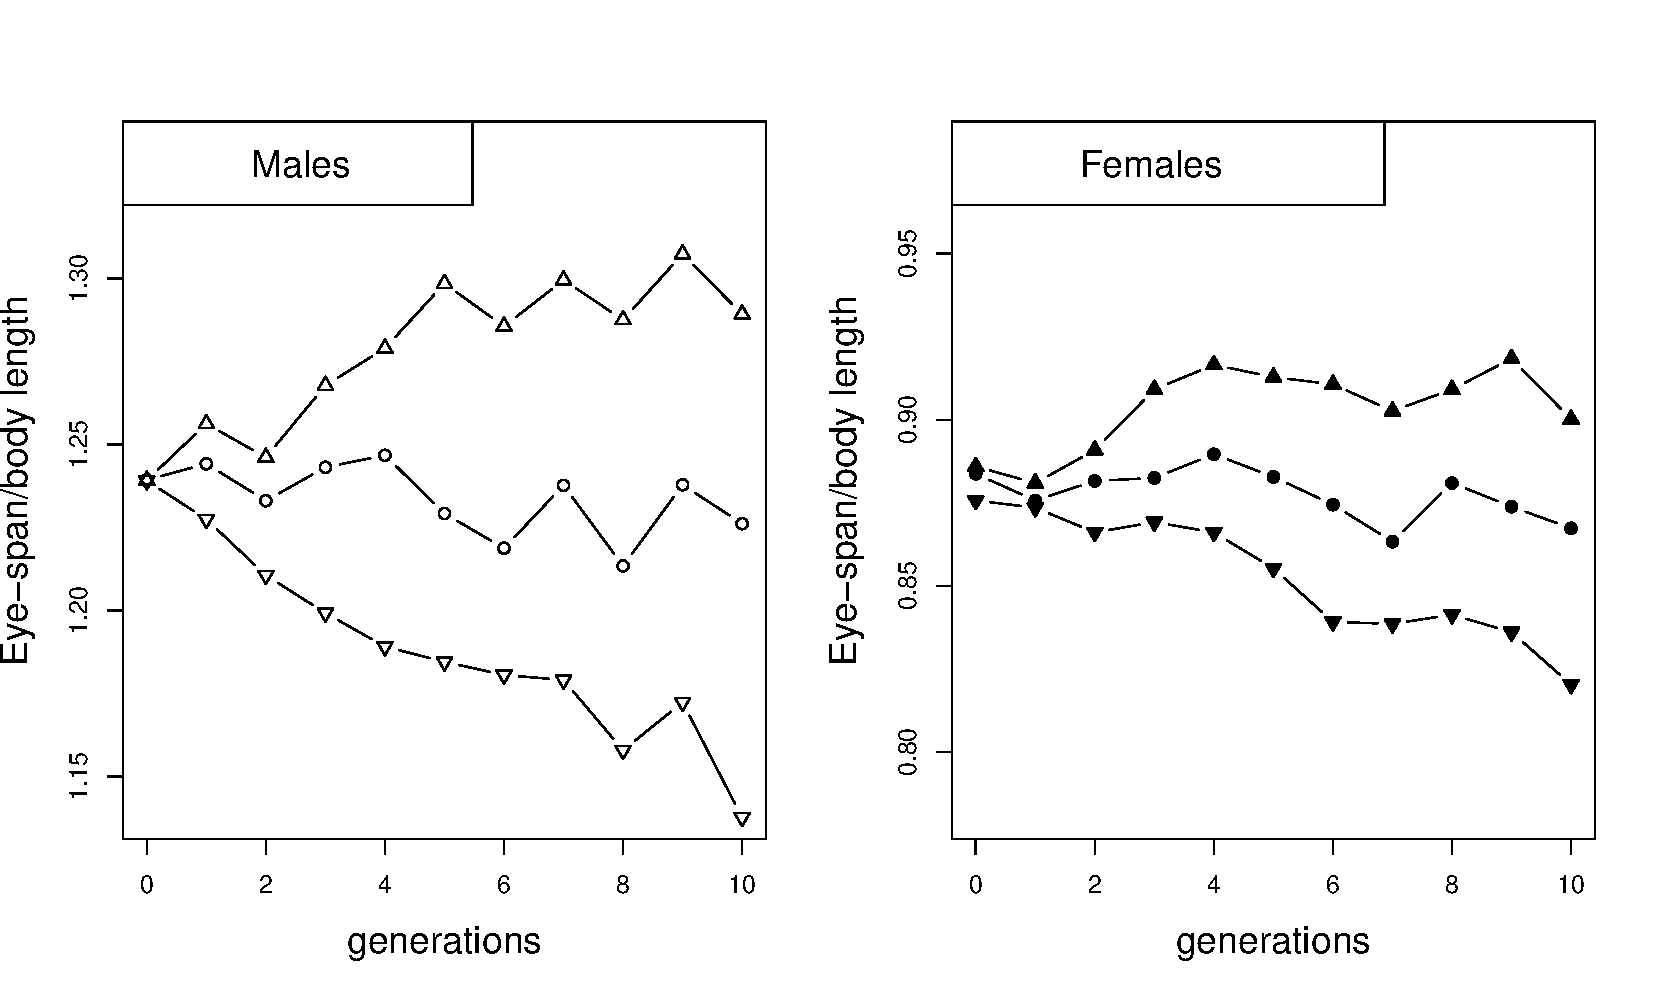
\includegraphics[width= \textwidth]{Journal_figs/Quant_gen/stalk_eyed_flies/stalk_eyed_flies_response.pdf}
\end{center}
\caption{ \citeauthor{wilkinson:93} selected two of populations for flies for
 increased and eye-stalk to body length ratio in males (mean shown as
 up triangles), and two for a
 decreased ratio (down triangles), by taking the top 10 males with the highest (lowest)
 ratio out of 50 measures. He also established two control populations
 (circles). He constructed each generation of females by sampling 10
 at random from each population.  

} \label{fig:Stalk_eyed_response}   %\cite{potti:11} 
\end{figure}


\begin{question}

At the end of ten generation in \citeauthor{wilkinson:93}'s experiment (Figure
\ref{fig:Stalk_eyed_response}) the males from the up- and down-selected
lines had mean eye-stalk to body ratios of $1.29$ and $1.14$
respectively. While the females from the up- and down-selected lines
had means of $0.9$ and $0.82$. \\
{\bf A)} \citeauthor{wilkinson:93} estimated that by selecting the top/bottom
10 males he had on average shifted the mean body ratio by 0.024 within
each generation. What is the male heritability of  mean eye-stalk to body ratio?

{\bf B} Assume that the heritability of male and female phenotypes are
equal.  Assuming that there is no direct
selection on female boy-ratios in this experiment, i.e. that all of
the response in female is due to correlated selection, can you
estimate the genetic correlation? 
\end{question}


\subsection{Some applications of the multivariate trait breeder's equation}

\paragraph{Hamiliton's Rule and the evolution of altruistic and
  selfish behaviours}

\graham{this is work in progress}
Adaptative evolution should push the population towards acting in a way that
maximizes their evolurionary fitness, subject to constraints. Yet individuals
frequently behave in ways that sacrific their own fitness for the
benefit of others. 
Hamilton supplied the first general explanation of such altruism.
His intuition was that while an individual is losing
out of some reproductive output, the alleles underlying an altruistic behaviour
can still spread in the population if this cost is outweighed by benefits gained 
through the transmission of these alleles through a related individual (note that this means that the
allele is not acting in an self sacrificing manner, even though
individuals may as a result). 
We can use our quantitative genetics framework to gain some simple
intuition for when altruistic behaviours should evolve through kin
selection. To do this we can derive a simple version of Hamilton's
Rule by thinking about the phenotypes of an individual's kin as
genetically correlated phenotype.

To do this we
can follow Queller's (1992) treatment, to rederive Hamiliton's rule in
a quantitative genetics framework (Hamilition original work did this in a
population genetics framework).

So lets imagine that individuals interact in pairs, with our focal
individual $i$ being paired with an individual $j$.  
Imagine that individuals have two possible phenotypes $X=1$ or $0$,
corresponding to providing or withholding some small act of `Altruism'
(we could just as easily flip these labels and call them a unselfish
act and a selfish act respectively). 
Our pairs of individuals interacting could for example being siblings sharing a
nest. The altruistic trait could be as simple as growing at a
slightly slower rates so as to reducing sibling-competition for food from
parents, or more complicated acts of altruism such as foregoing their
own reproduction so as to help their parents raise their siblings.

Providing the altruistic act has a cost $C$ to the fitness of our
individual, with failing to provide this act has no cost. Receiving this
altruistic act confers a fitness benefit $B$ (not receiving it has no benefit).
Hamiliton's Rule states that such a trait will spread through the
population if the average coefficient of relatedness between the
interactiong individuals is $r$, the average number of alleles that
our pairs of indviduals share identical by descent at a locus. We can express
Hamilton's rule as
\begin{equation}
 C<rB
\end{equation}

\begin{marginfigure}
\begin{center}
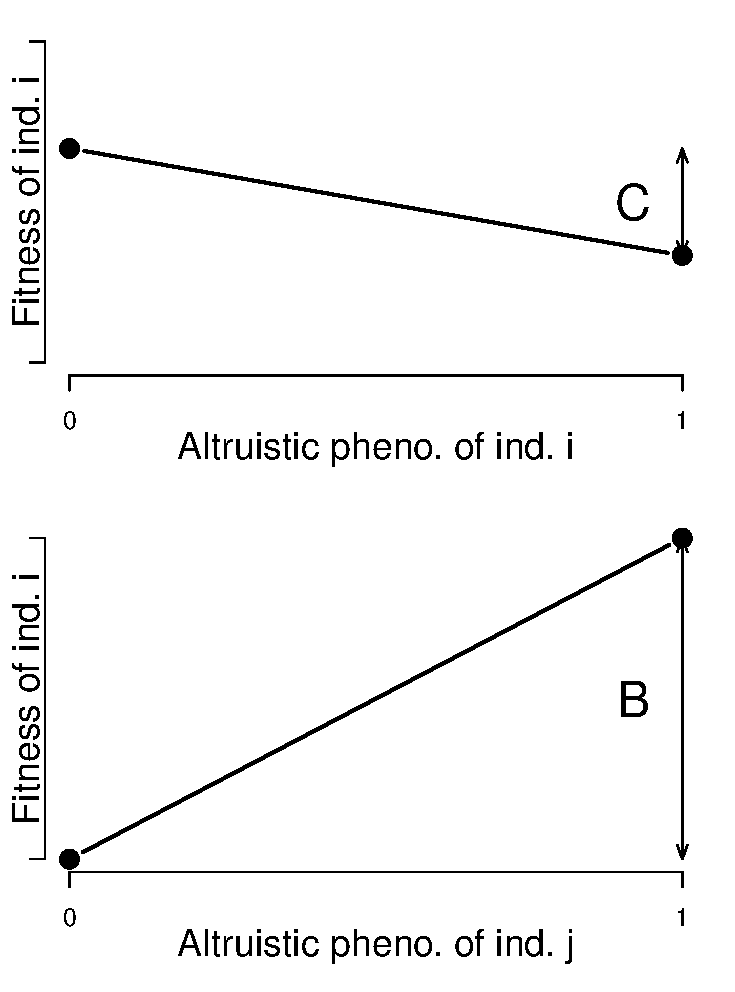
\includegraphics[width= \textwidth]{figures/Response_to_sel/Hamiltons_rule_B_C.pdf}
\end{center}
\caption{ } \label{fig:Hamilton_B_C}
\end{marginfigure}



To sketch a proof of this lets assume that our focal $i$ individual's relative fitness can be written as 
\begin{equation}
W(i,j)= W_0 + W_i +W_j
\end{equation}
where $W_i$ is the contribution of the fitness of the individual $i$ due
to this phenotype, and $W_j$ is the contribution to our
individual $i$'s fitness due to the $j$'s behaviour (i.e. phenotype).
With the benefit $B$ and cost $C$ our $W(i,j)$ are depicted in
Figure \ref{fig:Hamilton_B_C}. 

We can write the expected change in phenotype is 
\begin{equation}
R = \beta_i V_A + \beta_j V_{A,i,j}
\end{equation}
Our alturistic phenotype is increasing in the population if $R>0$,
i.e. if
\begin{eqnarray}
 0<& \beta_i V_A + \beta_j V_{A,i,j}  \nonumber  \\
-\beta_i < & \beta_j \frac{V_{A,i,j}}{V_A} 
\end{eqnarray}
So what's the average genetic covariance between
individual $i$ and $j$'s alturistic phenotype? Well the covariance of
the same phenotype between two individual's is just $2 F_{i,j} V_A$ (see \eqref{additive_covar_general_rellys}). our $F_{i,j}$ is the probability that an allele found in individual
$i$ is identical by descent to an allele drawn from $j$, $2 F_{i,j}$
can be interpreted as the average number of alleles shared between
individuals $i$ and $j$ our re. So 
\begin{eqnarray}
 -\beta_i < & \beta_j \frac{2 F_{i,j} V_A}{V_A} \nonumber  \\
-\beta_i < & \beta_j 2 F_{i,j} \nonumber  \\
C < & r  B \\
\end{eqnarray}


\paragraph{Sexual selection and the evolution of mate preference by Indirect benefits. }

Males ($\mars$) and females ($\venus$)

We will assume that there is a trait, e.g. tail length, is under direct
selection in males, such that its response to selection can be written as
\begin{equation}
R_{\mars} = \beta_{\mars} V_{A, \mars}
\end{equation}

Lets assume that the female preference trait is not under direct
selection $\beta_{\venus}=0$ then the response to selection of the
preference trait can be written as
\begin{eqnarray}
R_{\venus} &=\beta_{\venus}V_{A,\venus}  + \beta_{\mars} V_{A, \venus
  \mars}
& = \beta_{\mars} V_{A, \venus  \mars}
\end{eqnarray}
so the female preference will respond to selection if it is
genetically correlated with the male trait, i.e. if $V_{A, \venus
  \mars}$. There's a number of different ways this genetic correlation could arise. The
simplest is that the loci underlying the male trait may have a
pleiotropic effect on female preference, however, female preference
may often have quite a distinct genetic basis from male display traits.

A more general way in which trait-preference genetic correlations may
arise is through assortative mating. Females vary in their
tail-length preference, the ones will a preference for longer
tails will mate with long-tailed males and the opposite for females
with a preference for shorter-tails. Therefore, there will be a
correlation between mates display and preference traits (see Figure \ref{fig:assort_mating_2_trait}). 


\begin{figure}
\begin{center}
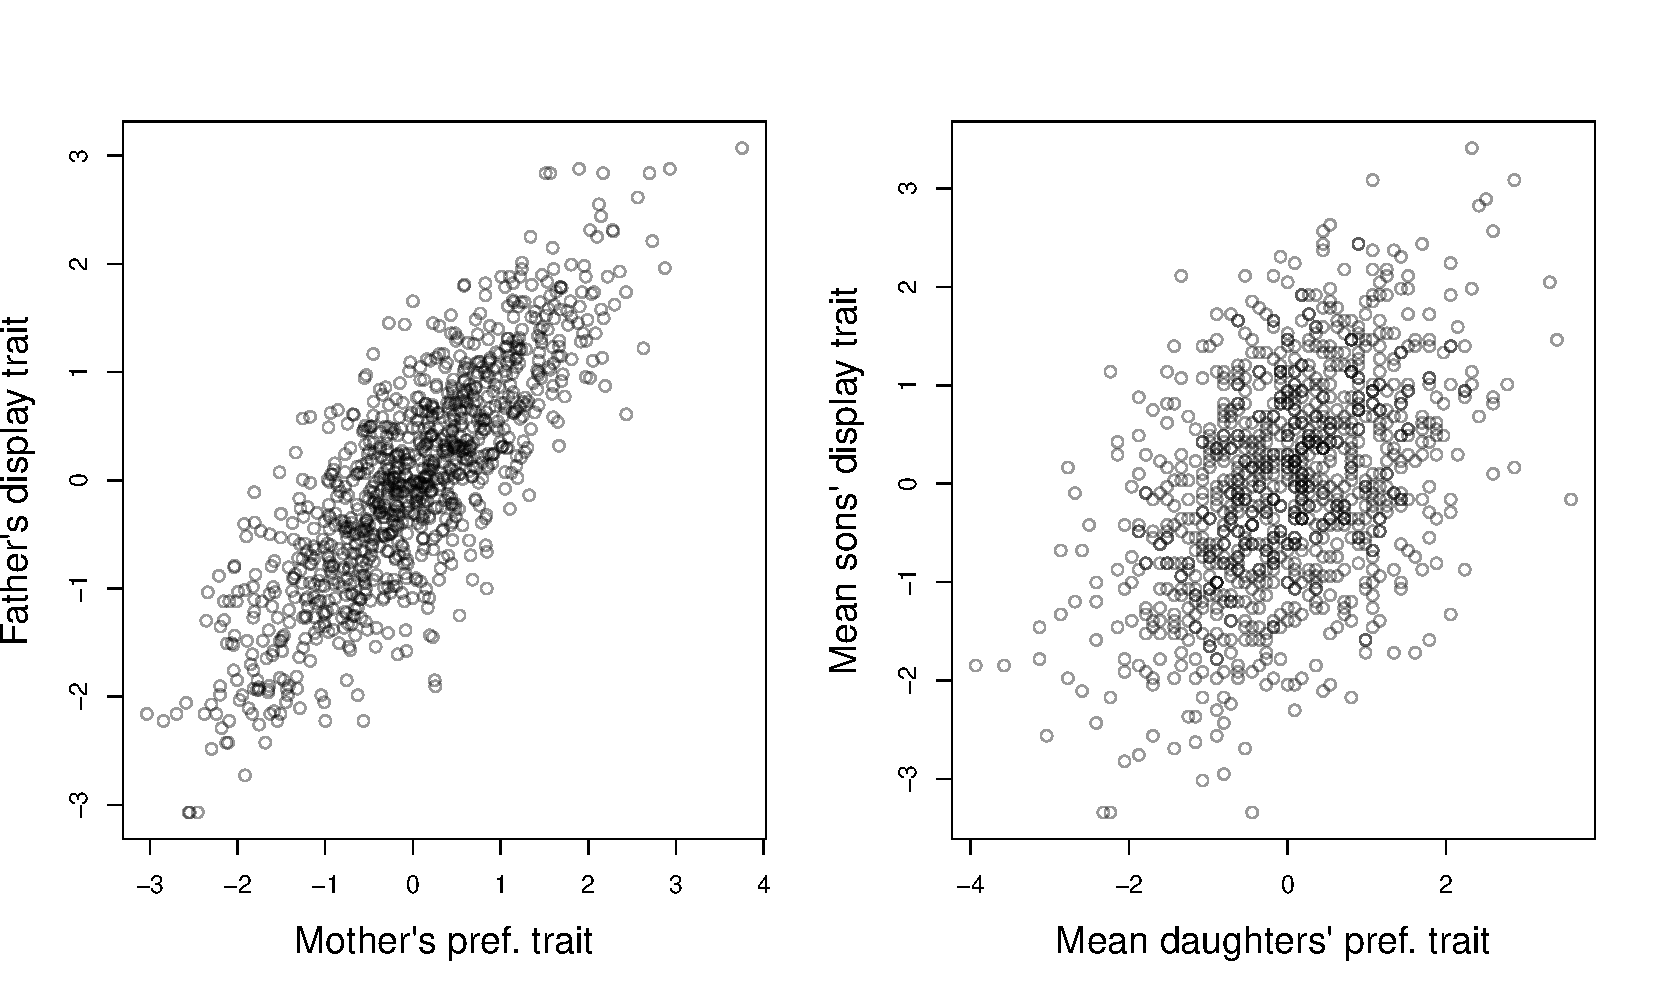
\includegraphics[width=\textwidth]{figures/Response_to_sel/Genetic_corr_assort_mating.pdf}
\end{center} \label{fig:assort_mating_2_trait}
\caption{}
\end{figure}

